\documentclass[11pt,xcolor=svgnames]{beamer}
\usepackage{dsfont,natbib,setspace,changepage,multirow}
\mode<presentation>

% replaces beamer foot with simple page number
\setbeamertemplate{navigation symbols}{}
\setbeamercolor{frametitle}{fg=black}
\newcommand{\theme}{\color{Maroon}}

\setbeamertemplate{footline}{
   \raisebox{5pt}{\makebox[\paperwidth]{\hfill\makebox[20pt]{\color{gray}\scriptsize\insertframenumber}}}}

\usepackage{tikz}
  
\graphicspath{{/green/Dropbox/inputs/},
{/Users/mtaddy/Dropbox/inputs/},
{/home/taddy/teaching/datamining/graphs/},
{/home/taddy/project/bigdata/graphs/},
{/Users/mtaddy/project/bigdata/graphs/}}

\setbeamercolor{whitebox}{bg=gray!10}

% colors
\newcommand{\bk}{\color{black}}
\newcommand{\rd}{\color{red}}
\newcommand{\fg}{\color{ForestGreen}}
\newcommand{\bl}{\color{blue}}
\newcommand{\gr}{\color{black!60}}
\newcommand{\sg}{\color{DarkSlateGray}}
\newcommand{\br}{\color{SaddleBrown}}
\newcommand{\nv}{\color{Navy}}


% common math markups
\newcommand{\bs}[1]{\boldsymbol{#1}}
\newcommand{\mc}[1]{\mathcal{#1}}
\newcommand{\mr}[1]{\mathrm{#1}}
\newcommand{\bm}[1]{\mathbf{#1}}
\newcommand{\ds}[1]{\mathds{#1}}
\newcommand{\indep}{\perp\!\!\!\perp}

% spacing and style shorthand
\setstretch{1.1}

% shorthand
\newcommand{\sk}{\vspace{.5cm}}
\newcommand{\R}[1]{{\tt \nv #1}}
\newcommand{\til}{{\footnotesize$\bs{\stackrel{\sim}{}}$}}
\DeclareSymbolFont{extraup}{U}{zavm}{m}{n}
\DeclareMathSymbol{\vardiamond}{\mathalpha}{extraup}{87}

\begin{document}

\setcounter{page}{0}
%\setbeamercolor{background canvas}{bg=gray!05}
{% \usebackgroundtemplate{
\includegraphics[height=\paperheight]{phoenix}}
\begin{frame}[plain]
\begin{center}


{\bf \Large [9] Big Data: Trees}

\vskip 1.5cm 
Matt Taddy, University of Chicago Booth School of Business

\vskip .2cm 
\texttt{faculty.chicagobooth.edu/matt.taddy/teaching} 


\end{center}
\end{frame} }


\begin{frame}

{\nv Decision Trees:} {Using tree-logic to make predictions.}

\sk
~~~~{\theme CART:} Classification and Regression Trees.

\vskip .1cm
~~~~{\theme Random Forests:} averaging over many possible trees.

\sk
Simple examples: \bk NBC, prostate cancer, motorcycle crashes.


\vskip .1cm
Larger example on house prices in california.



\end{frame}


\begin{frame}
{What is a Decision Tree?}

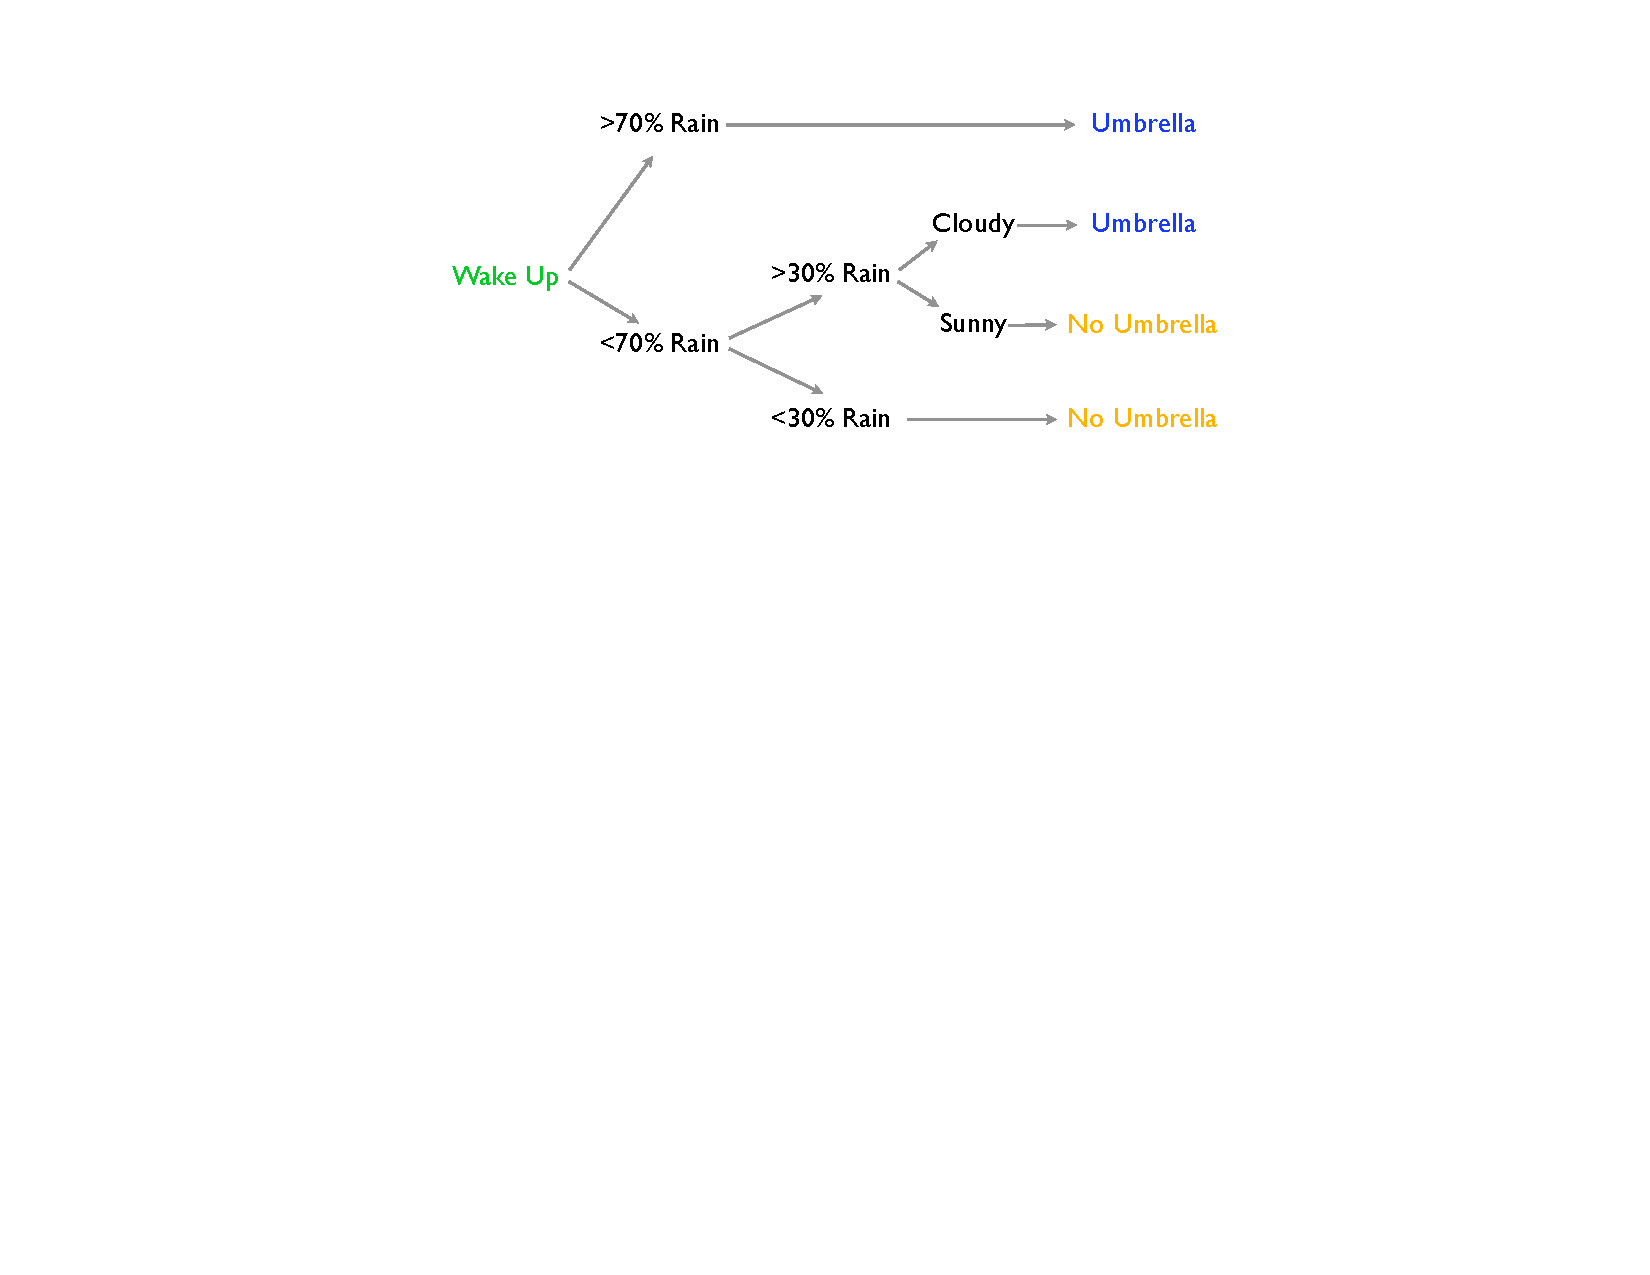
\includegraphics[width=4.25in]{../graphs/umbrella}


\vskip .3cm
\bk Tree-logic uses a series of steps to come to a conclusion.\\
 The trick is to have mini-decisions combine for good choices.
\\ Each decision is a node, and the final prediction is a {\theme
  leaf node}

\end{frame}



\begin{frame}

{\bf Decision Trees are a Regression Model}

\sk
You have inputs $\bm{x}$ {\gr (forecast, current conditions)} \\ and an output of
interest $y$ {\gr (need for an umbrella)}.


\sk 
Based on previous data, the goal is to specify branches of \\ choices 
that lead to good predictions in new scenarios.


{In other words, you want to estimate a {\nv Tree Model}.}


\sk
\bk
Instead of linear coefficients, we need to find `{\theme decision nodes}': \\~~~split-rules defined via thresholds on some dimension of 
$\bm{x}$.

\vskip .5cm
Nodes have a parent-child structure: every node except the root has a parent, and every node except the leaves has two children.


\end{frame}


\begin{frame}

{\bf Decision trees are like a game of mousetrap}

\vskip .25cm
You drop your $\bm{x}$ covariates in at the top, and each decision node
bounces you either left or right.  Finally, you end up in a {\theme leaf node} which contains the data subset defined by these decisions (splits).


\begin{equation*}
\begin{array}{ccccc}
& &  \hskip -2.2cm x_i = 0 &&\\
& & \hskip -2.3cm \swarrow ~~~\searrow &&\\
&  \hskip -.8cm x_j = 2 & & \hskip -2.3cm \{\bm{x}: x_i>0\}&\\
& \hskip -.7cm \swarrow~~~\searrow & & &\\
\{\bm{x}: x_i \leq  0, x_j \leq  2\}& & \hskip -.5cm \{ \bm{x}: x_i \leq 0, x_j>2 \}& &
\end{array}
\end{equation*}

\vskip .5cm
The {\nv prediction rule} at each leaf (a class probability or predicted $\hat y$) is  the average of the sample $y$ values that ended up in that leaf.

\end{frame}



\begin{frame}


{\bf  Estimation of Decision Trees}

\sk  As usual, we'll maximize data likelihood 
  (minimize  deviance).

\vskip .1cm
{\gr But what are the observation probabilities in a  tree model?}

\sk\bk Two types of likelihood: { classification} and {regression} trees.

\vskip .1cm
~~~~~ A given covariate $\bm{x}$ dictates your path
through \\
~~~~~ tree nodes, leading to a {\theme leaf node} at the end.

\sk\bk
{\nv Classification trees} have {\theme class probabilities} at the leaves.\\
{\gr Probability I'll be in heavy rain is 0.9 (so take an umbrella).}

\vskip .25cm
 
{\nv Regression trees} have a {\theme mean response} at the leaves.\\
{\gr The expected amount of rain is 2in (so take an umbrella).}

\end{frame}

\begin{frame}

{\bf Tree deviance is the same as in linear models}


\vskip .5cm
{Regression Deviance:} $\sum_{i=1}^n(y_i - \hat{y}_i)^2$

\vskip .25cm
{Classification Deviance:} 
$- \sum_{i=1}^n\log(\hat{p}_{y_i})$ 

\vskip .1cm{\gr
It is also common to use Gini Deviance, $- \sum_{i=1}^n\hat{p}_{y_i}(1-\hat{p}_{y_i})$}


\sk
Instead of being based on $\bm{x}'\bs{\beta}$, predicted $\hat{p}$ and $\hat{y}$  are\\
functions of $\bm{x}$ passed through the decision nodes.

\sk \bk
We need a way to estimate the sequence of decisions.
\begin{itemize}
\item How many are they?  What is the order?
\end{itemize}
There is a {\it huge} set of possible tree configurations.

\end{frame}

\begin{frame}

Given a {\nv parent} set of data $\{\bm{x}_i,y_i\}_{i=1}^n$, the {\theme optimal split}
is that location $x_{ij}$ on some dimension $j$ on some observation $i$, so that the {\nv child} sets 
\[
\text{\rm{left}:}~\{\bm{x}_k,y_k:~x_{kj} \leq x_{ij}\}
\text{~~and~~\rm{right}:}~\{\bm{x}_k,y_k:~x_{kj} > x_{ij}\}
\]
are as homogeneous in response $y$ as possible.

\vskip .5cm
For example, we will minimize the sum of squared errors \\
\[
\sum_{k \in \mathrm{left}} (y_k - \bar y_{\mathrm{left}})^2 + \sum_{k \in \mathrm{right}} (y_k - \bar y_{\mathrm{right}})^2
\]
for {\it regression trees}, or gini impurity  for {\it classification trees} \\(e.g., the sum across children `c' of $n_{\mathrm{c}}\bar y_{\mathrm{c}}(1-\bar y_{\mathrm{c}})$ if $y\in \{0,1\}$).

\end{frame}

\begin{frame}


{\bf We estimate decision trees by being recursive and greedy}


\vskip .5cm
{\nv CART} grows the tree through a sequence of splits:

\vskip .25cm
\begin{itemize}
\item Given any set (node) of data, you can find the {\theme optimal split} (the error minimizing split) and divide into two child sets.
\item 
We then look at each child set, and again find the optimal split to divide it into two homogeneous subsets.
\item
The children become  parents, and we look again for the optimal split on their new children (the grandchildren!).
\end{itemize}

\vskip .25cm
You stop splitting and growing when the size of the leaf nodes hits some minimum threshold (e.g., say no less than 10 obsv per leaf).

{\gr Often there are also
minimum deviance improvement thresholds.}
\end{frame}



\begin{frame}

{\bf Use the {\nv tree} library for CART in R}

\sk
The syntax is essentially the same as for {\tt glm}:

\vskip .1cm
\R{\small mytree = tree(y \til x1 + x2 + x3 ..., data=mydata)}

\sk
There are only a few other possible arguments, \\
all of which dictate possible types of new children
\begin{itemize}
\item \R{mincut} is the minimum size for a new child.
\item \R{mindev} is the minimum (proportion) deviance improvement for
  proceeding with a new split.
\end{itemize}
{These are important: you may want to make them smaller\\ than their defaults: {\tt mincut=5}, {\tt mindev=0.01}.}

\vskip .3cm
As usual, you can \R{print}, \R{summarize}, and \R{plot} the tree.
\end{frame}

\begin{frame}[fragile]


\begin{adjustwidth}{-.2in}{}

{\bf \theme Recall our NBC data:} {\bf  viewer
demographic \% by show.}

\sk
Consider a classification tree to predict genre from demographics.
\vskip .2cm
{\sg \scriptsize
\begin{verbatim}
> genretree
node), split, n, deviance, yval, (yprob)
      * denotes terminal node
\end{verbatim}

\vskip .2cm
\nv
\begin{semiverbatim}
1) root 40 75.800 Drama/Adventure ( 0.475 0.425 0.100 )  
 2) CABLE.W.O.PAY < 28.6651 22 33.420 Drama/Adventure (0.73 0.09 0.18)  
  4) VCR.OWNER < 83.749 5  6.730 Situation Comedy (0.00 0.40 0.60) *
  5) VCR.OWNER > 83.749 17  7.606 Drama/Adventure (0.941 0.000 0.059)  
   10) TERRITORY.EAST.CENTRAL < 16.4555 16  0.000 Drama/Adventure(1 0 0) *
   11) TERRITORY.EAST.CENTRAL > 16.4555 1  0.000 Situation Comedy(0 0 1) *
  3) CABLE.W.O.PAY > 28.6651 18 16.220 Reality ( 0.16667 0.83333 0 )  
    6) BLACK < 17.2017 15  0.000 Reality ( 0 1 0 ) *
    7) BLACK > 17.2017 3  0.000 Drama/Adventure ( 1 0 0 ) *
\end{semiverbatim}}


\end{adjustwidth}

\vskip .25cm
Output from \R{tree} shows a series of decision nodes and
the proportion in each genre at these nodes, down to the leaves.

\end{frame}
   
\begin{frame}

{\bf Trees are easiest to understand in a {\theme dendrogram}}

\vskip -.3cm

\hskip -.2in
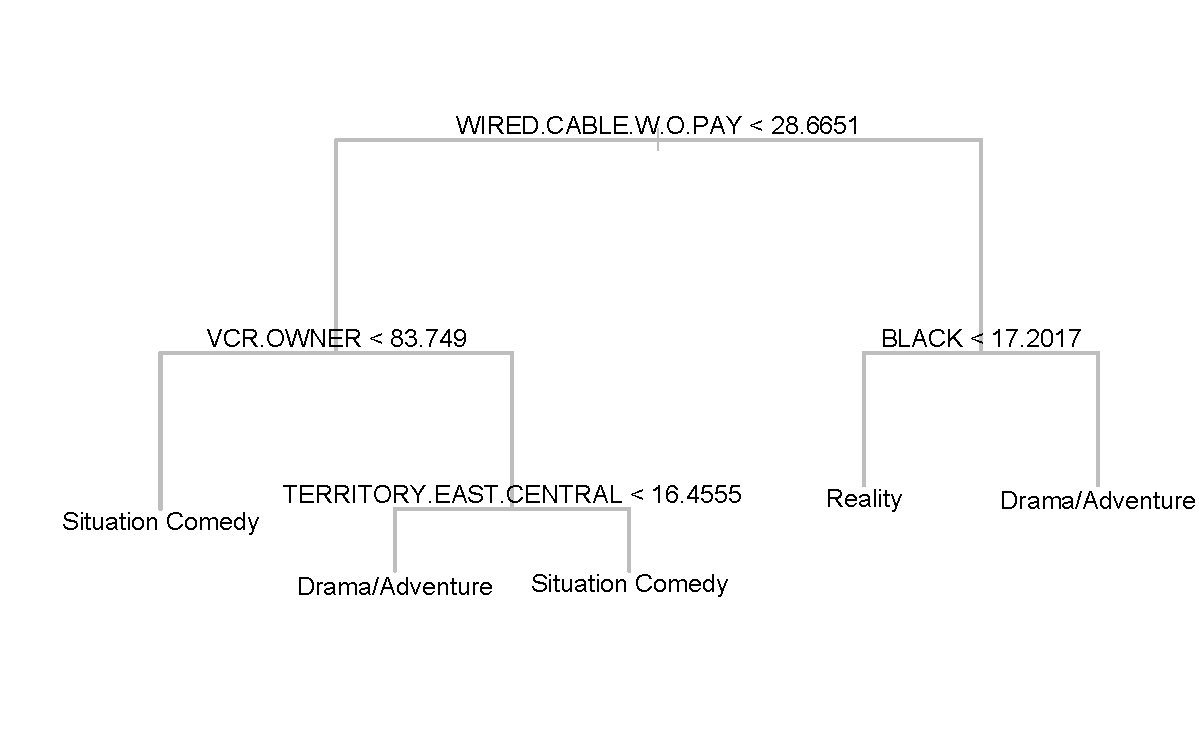
\includegraphics[width=4.45in]{../graphs/NBCgentree}

\vskip -.5cm\small
Shows the sequence of internal splits, ending in leaf-node
decisions.\\
 Here, the decision is the genre of highest
proportion in each leaf.\\\gr
To get the dendrogram, do \R{plot(mytree)} then \R{text(mytree)}.

\end{frame}



\begin{frame}[fragile]


Consider predicting {\theme engagement} from {\theme ratings} and {\theme
  genre}.

\vskip .25cm
Split on genre by turning it into a group of numeric variables:

{\nv \footnotesize \vspace{-.25cm}
\begin{verbatim} 
    x <- model.matrix(PE ~ Genre + GRP, data=nbc)[,-1]
    names(x) <- c("reality","comedy","GRP")
\end{verbatim}
  }\vspace{-.25cm}
{ We have a reference factor level ({\tt drama})}

\sk
{A regression tree:} 
{\small
\nv
\begin{verbatim}
       nbctree <- tree(PE ~ ., data=x, mincut=1)
\end{verbatim}}

Instead of genre, leaf predictions are expected engagement.

\vskip .25cm
{\tt mincut=1} allows for leaves containing a single show,
\\ with expected engagement that single show's PE.
\vskip -.25cm
\end{frame}

\begin{frame}

{\bf An NBC Show Engagement Tree}

\sk
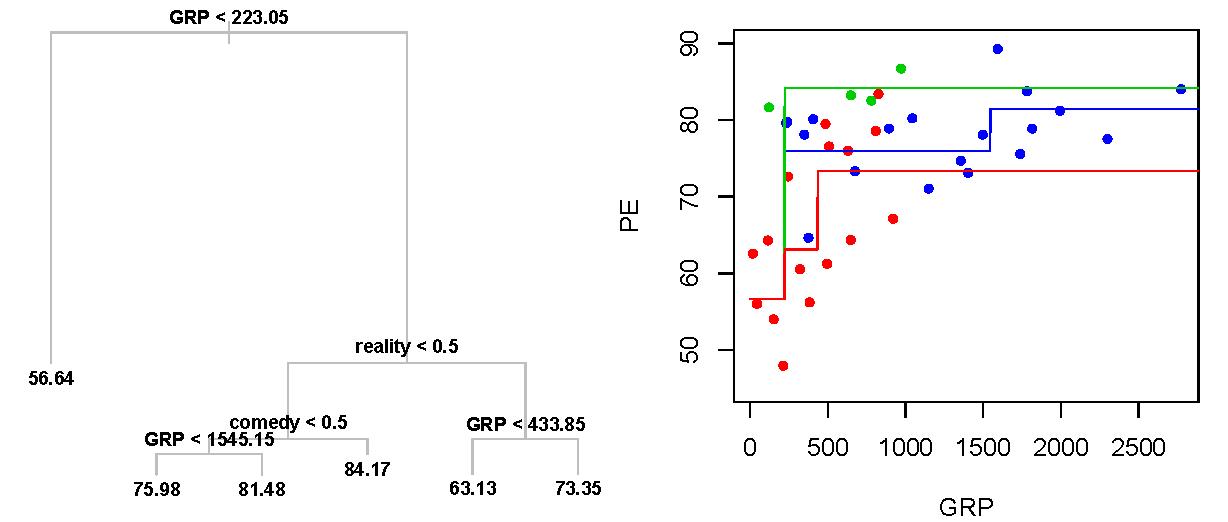
\includegraphics[width=4.25in]{../graphs/NBCtree}

\sk
{\fg Green is comedy}, {\nv blue is drama}, {\theme red is reality}\\
Nonlinear: PE increases with GRP, but in jumps\\
\gr Follow how the tree translates into changing $\ds{E}[{\tt PE}]$

\end{frame}

\begin{frame}

{\bf Trees provide \theme Automatic  Interaction Detection}

\sk
 For example, 
different genres are more/less dependent on GRP.

\vskip .25cm

 AID was an original motivation for building decision trees.  \\Older algorithms have
it in their name: CHAID, US-AID, ...

\sk
This is pretty powerful technology: \bk nonlinearity and \\ interaction
without having to specify it in advance.\\
 Moreover, nonconstant variance is no problem.

\vskip .25cm

Methods with these characteristics are called {\theme
  nonparametric}.\\
{\gr No assumed parametric model (eg, $y=x\beta + \varepsilon,
  ~\varepsilon \sim \mr{N}(0,\sigma^2)$).}


\end{frame}

\begin{frame}

{\bf \theme Pruning \bk your tree for cross validation}

\sk
Biggest challenge with such flexible models is avoiding overfit.\\
\bk For CART, the usual solution is to rely on cross validation.


\sk
The basic constraints {\sg ({\tt mincut, mindev})} lead to a full tree
fit.\\
 \nv Prune \bk this tree by removing split rules from the bottom
 up:

\vskip .2cm

~~~~At each step, remove the split that contributes  least to\\
~~~~deviance reduction, thus reversing CART's growth process.

\vskip .2cm\nv
Pruning yields candidate trees, and we use CV to choose.

\bk
Each prune step produces a candidate tree model, and we \\can compare
their out-of-sample prediction performance.

\end{frame}
 
\begin{frame}

{\bf Example: \theme Prostate Cancer Prognosis}

\sk
After tumor detection, there are many treatment options.
\begin{itemize}
\item Various chemo + radiation,  surgical removal.
\end{itemize}

\sk
Biopsy information is available to help in deciding treatment
\begin{itemize}
\item {\nv Gleason Score}: microscopic pattern classes.
\item {\nv Prostate Specific Antigen}: protein production.
\item {\nv Capsular Penetration}: reach of cancer into gland lining.
\item {\nv Benign Prostatic Hyperplasia Amount}: size of prostate.
\end{itemize}
Another influential variable is the patient's {\nv age}.

\sk
{The goal is to predict tumor log-volume (size, spread).}

\vskip -.5cm
\end{frame}


\begin{frame}

{\bf Full tree fit to 97 prostate cancer patients }

\vspace{-1cm}
\begin{adjustwidth}{-.3in}{}
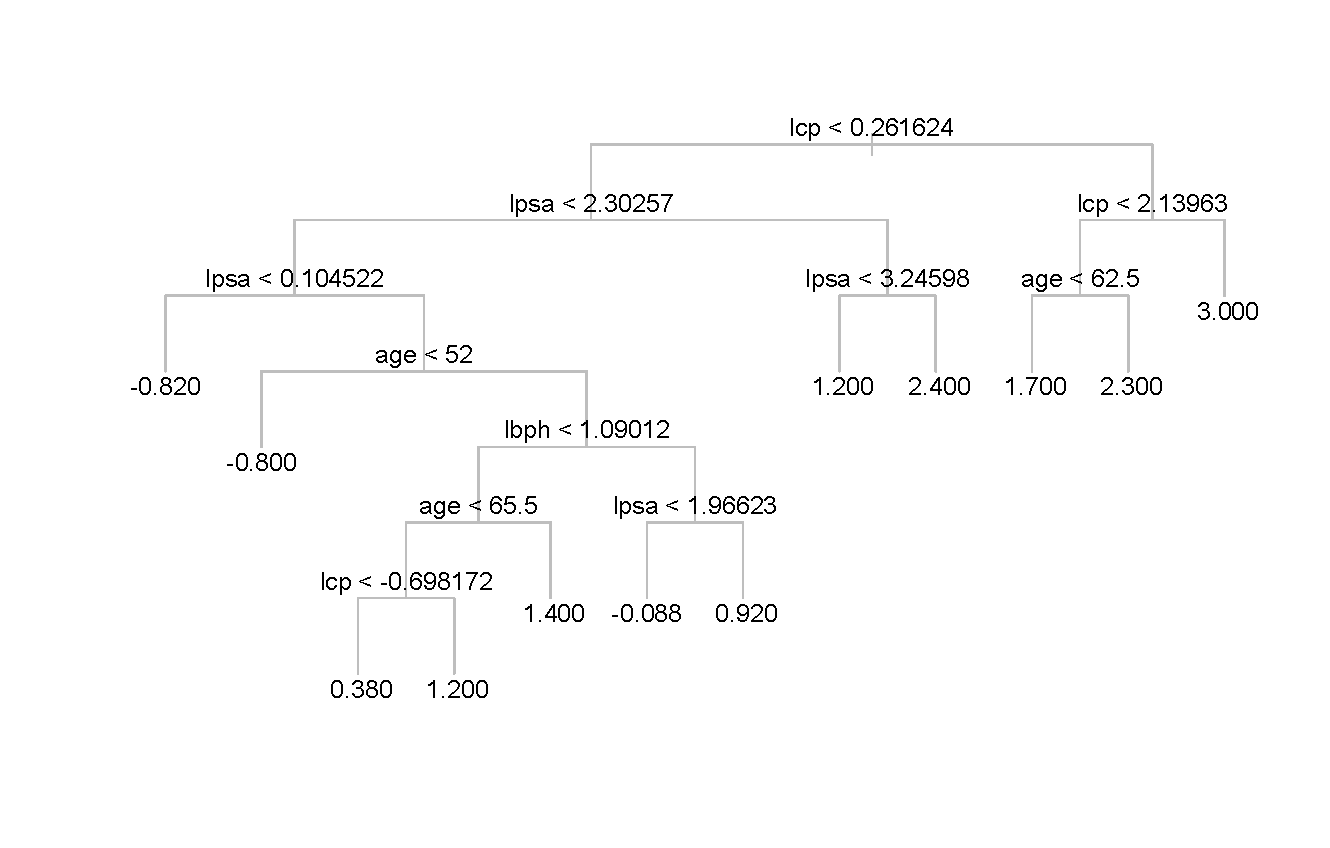
\includegraphics[width=4.75in]{../graphs/PSTtree}
\end{adjustwidth}

\vspace{-1cm}
Leaf node labels are expected tumor {\tt log(volume)}.\\
 Do we need all the splits?  Is the tree just fitting noise?
\end{frame}


\begin{frame}

{\theme \bf Cross-Validated Tree Pruning}


\vskip .25cm
{\tt cv.tree} does cross-validation across pruning levels.\\
\R{cvpst <- cv.tree(pstree, K=90) \theme \# K is nfolds}

\vskip -.25cm
\hskip 1.5cm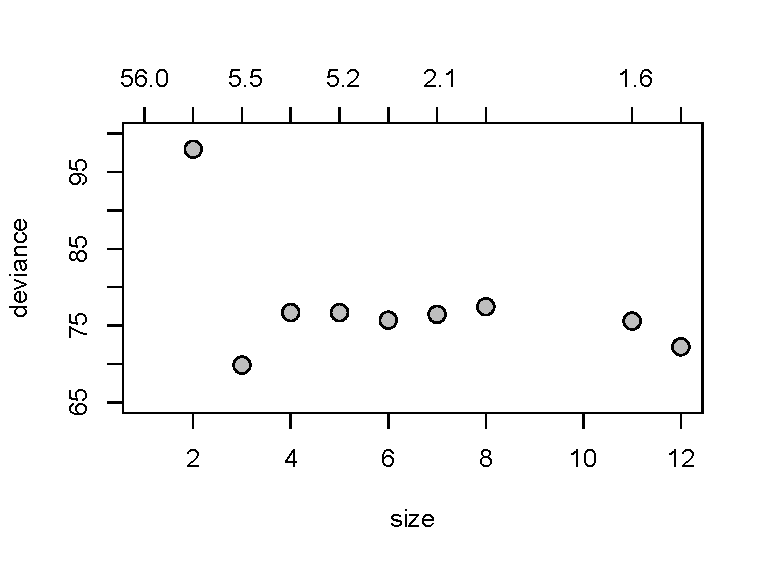
\includegraphics[width=3in]{../graphs/PSTcv}

\bk
The output can be plotted, and it holds out-of-sample deviance
for each tree size (the number of leaf nodes).
\vskip -.25cm


\end{frame}

\begin{frame}[fragile]

{\bf \gr Pruning the Prostate Cancer Tree}

\sk
Out-of-sample deviance can be used to choose tree size.
{\nv \footnotesize 
\begin{verbatim}
           > cvpst$size
            [1] 12 11  8  7  6  5  4  3  2  1
           > cvpst$dev
            [1] 72  75  77  76  76  77  77  70  97 160
\end{verbatim}}

Since size 3 has lowest CV deviance, it is `{\theme best}'.

\vskip .25cm
\sg To fit this tree, use the {\tt prune.tree} function:

\hfill \R{pstcut <- prune.tree(pstree, best=3)~~~~~~~~}

\hfill \gr {\tt pstcut} is then itself a new  tree object.


\end{frame}

\begin{frame}

{\bf \theme The Pruned Treatment Tree}

\vspace{-.5cm}
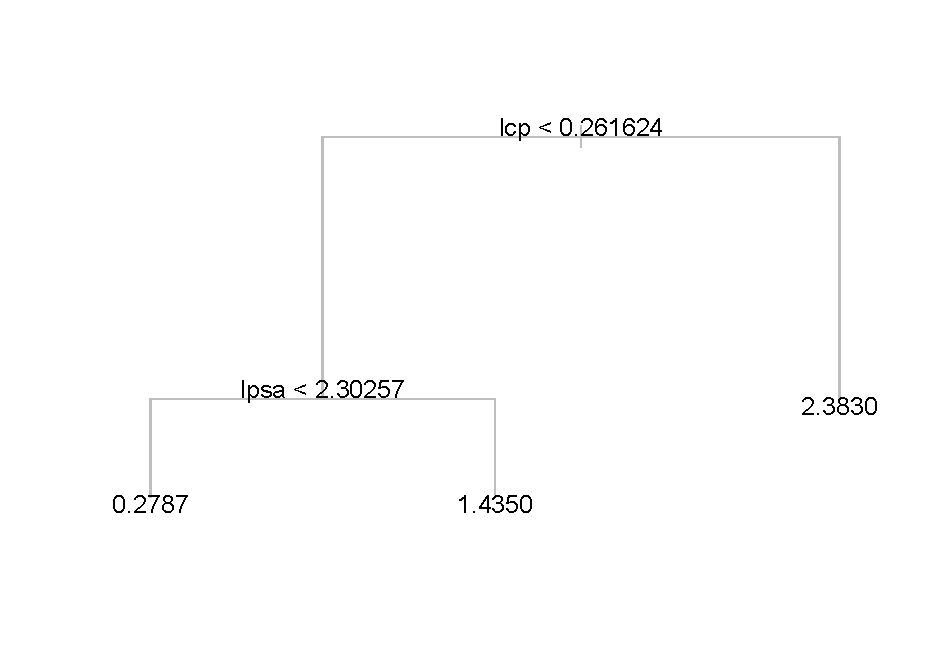
\includegraphics[width=4in]{../graphs/PSTcut}

\vspace{-.75cm}
CV chooses PSA and penetration as deciding variables.\\
 Note the interaction: penetration effect depends on PSA.
\end{frame}



\begin{frame}

{\bf \theme Prostate Cancer Prognosis Tree}

\vspace{-.5cm}
~~~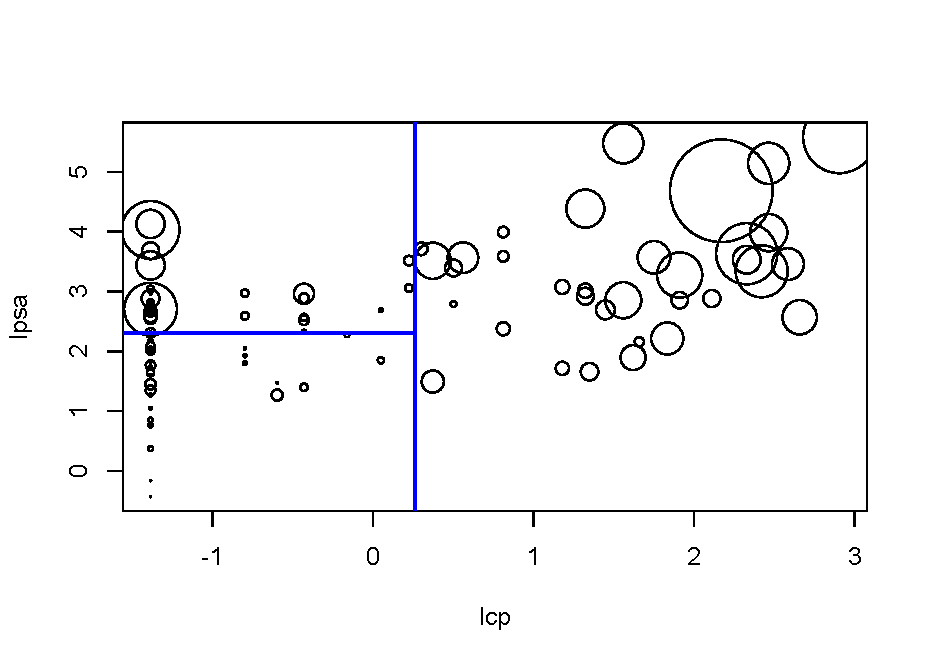
\includegraphics[width=4in]{../graphs/PSTfit}


With only 2 relevant inputs, we can plot the data and tree fit.
\\ Points proportional to tumor size,
leaf partitions are in blue.

\vskip -.25cm
\end{frame}




\begin{frame}


{\bf  Trees are awesome}

\vskip .25cm 
They automatically learn non-linear response functions
\\ and will discover interactions between variables.

\vskip .25cm
Example: Motorcycle Crash Test Dummy Data

\sg
$x$ is time from impact, $y$ is acceleration on the helmet.

\vspace{-1cm}
\begin{adjustwidth}{-.3in}{}
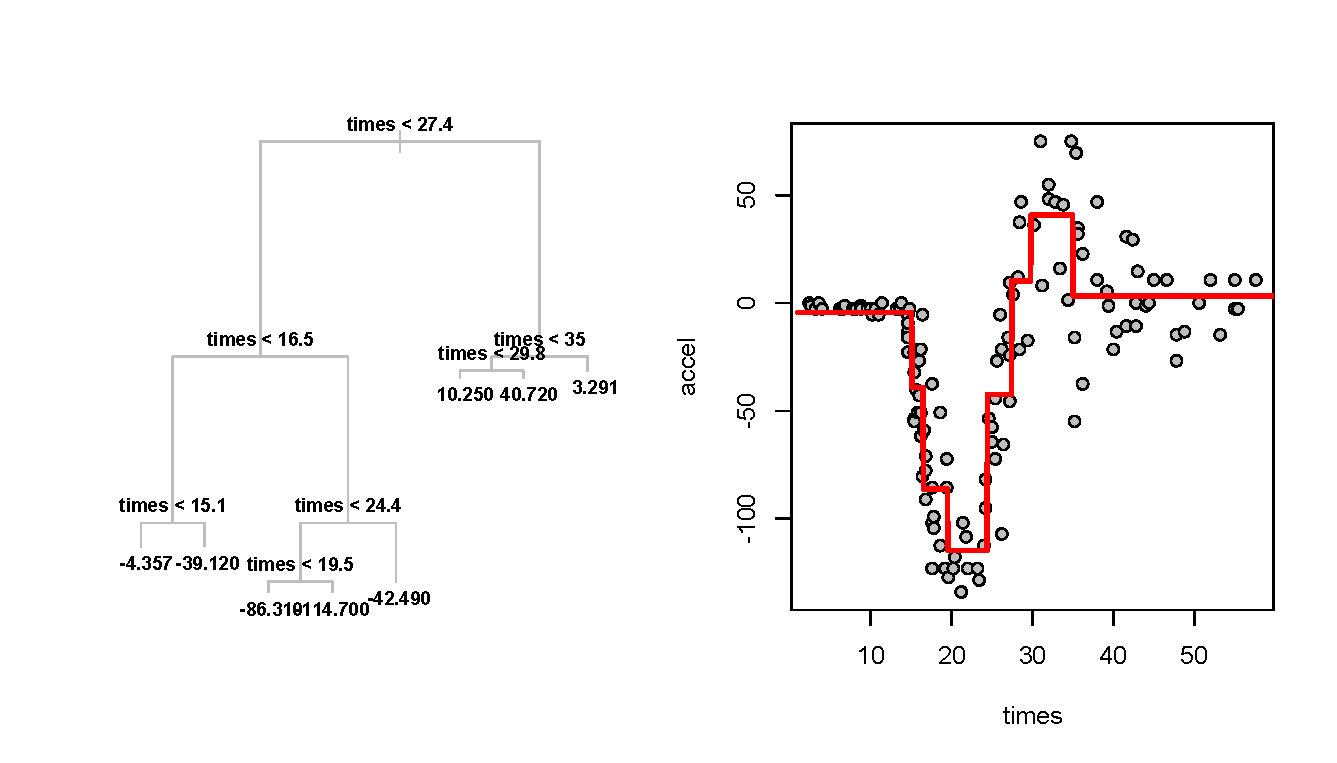
\includegraphics[width=4.6in]{../graphs/MCtree}
\end{adjustwidth}

\vskip -.75cm
\end{frame}


\begin{frame}

{Unfortunately, it is tough to avoid overfit with CART:}

\vskip .1cm \bk
Deep tree structure is so unstable that optimal depth is not easily chosen via cross validation, and there's no theory to fall back on.

\vskip .5cm \bk
Instead, we can average over a {\nv bootstrapped} sample of trees:  

\begin{itemize}
\item repeatedly re-sample the data, {\nv with-replacement}, \\to get a `jittered' dataset of $n$ observations.
\item for each resample, {\nv fit a CART tree}.
\item when you want to predict $y$ for some $\bm{x}$, \\take the {\nv average} prediction from this forest of trees.
\end{itemize}
Real structure that persists across datasets shows up in the average.  Noisy useless signals will average out to have no effect. 

\sk
{\bf \theme \hfill This is a Random Forest}
\end{frame}

\begin{frame}

{\bf \theme Random Forests}

\bk
\vskip .25cm
$\bullet$ Sample $B$ subsets of the data {\tt +} variables: \\ ~~~e.g., 
observations $1,5,20,...$ and inputs $2,10,17,...$

\vskip .2cm
$\bullet$ Fit a tree to each subset, to get $B$ fitted trees is $\mc{T}_b$.

\vskip .2cm
$\bullet$
Average prediction across trees:

\vskip .1cm
 ~~~~ -  for regression average $\ds{E}[y|\bm{x}] = \frac{1}{B}\sum_{b=1}^B \mc{T}_b(\bm{x})$.

 \vskip .1cm
 ~~~~ -  for classification let $\{\mc{T}_b(\bm{x})\}_{b=1}^B$ vote on $\hat y$.

\vskip .25cm
{\gr The observation resample is usually {\it with-replacement}, so that this is taking the {\it average of bootstrapped trees} (i.e., `bagging')}

\end{frame}

\begin{frame}

{\bf Understanding \theme Random Forests}

\sk Recall how CART is used in practice.
\begin{itemize}
\item Split to lower deviance until leaves hit minimum size.
\item Create a set of candidate trees by pruning back from this.
\item Choose the best among those trees by cross validation.
\end{itemize}

\sk {\nv Random Forests avoid the need for CV.}

\vskip .1cm Each tree `$b$' is not overly complicated 
because \\you only work with a  limited set of variables.

\vskip .1cm Your predictions are not `optimized to noise' 
because \\they are averages of trees fit to many different subsets.

\sk
RFs are a great go-to model for nonparametric prediction.
%\\{\gr As with all trees, they're not great in high ($>100$) dimension.}

\end{frame}

\begin{frame}[fragile]

{\bf Model Averaging}

\sk
This technique of `{\nv Model Averaging}' is central to \\many advanced
nonparametric learning algorithms.

\vskip .1cm
{\gr ensemble learning, mixture of
experts, Bayesian averages, ...}\\

\vskip .1cm
It works best  with flexible but simple models

\sk
Recall lasso as a stabilized 
version of stepwise regression \\(if you jitter the data your
estimates stay pretty constant).

\vskip .1cm 
Model averaging is a way to take arbitrary {\it unstable} methods, 
and make them stable.  {\theme This makes training easier.}



\sk\gr
Probability of rain on a new day is the average P(rain)\\
across some trees that split on forecast, others on sky.\\
\bk We don't get tied to one way of deciding about umbrellas.

\end{frame}


\begin{frame}[fragile]

{\bf Random Forests in R}

\vskip .25cm

R has the {\tt randomForest} package, \\which
works essentially the same as {\tt tree}

\vskip .1cm{\small \nv
~~~~\verb|spamrf <- randomForest(spam ~ ., data=xemail)|
}
\vskip .25cm 
{\gr For big datasets, use ${\tt x = x,  ~y=y}$ like in {\tt gamlr}}.


\sk
{\nv Unfortunately, you lose
the interpretability of a single tree.}

However, if you set {\tt importance=TRUE}, {\tt Random Forest}
will evaluate each $\mc{T}_b$'s performance on the {\it left-out sample}
(recall each tree is fit on a sub-sample).  This yields nice OOS stats.

\vskip .25cm
They can be slow (due to many tree fits) but\\
they can also be fit in parallel or on distributed data...

\end{frame}



\begin{frame}


\begin{center}

\includegraphics[width=.75\textwidth]{../graphs/MCtreedraw}
\end{center}

\vskip -.25cm
Fitting CART to sampled-with-replacement data is equivalent to randomly {\nv weighting} your observations in the deviance calculations. 

\hfill {\gr (size proportional to weight in this picture)}.

\end{frame}

\begin{frame}

{\bf \theme Random Trees \bk for the Motorcycle Data}


\vspace{-1cm}
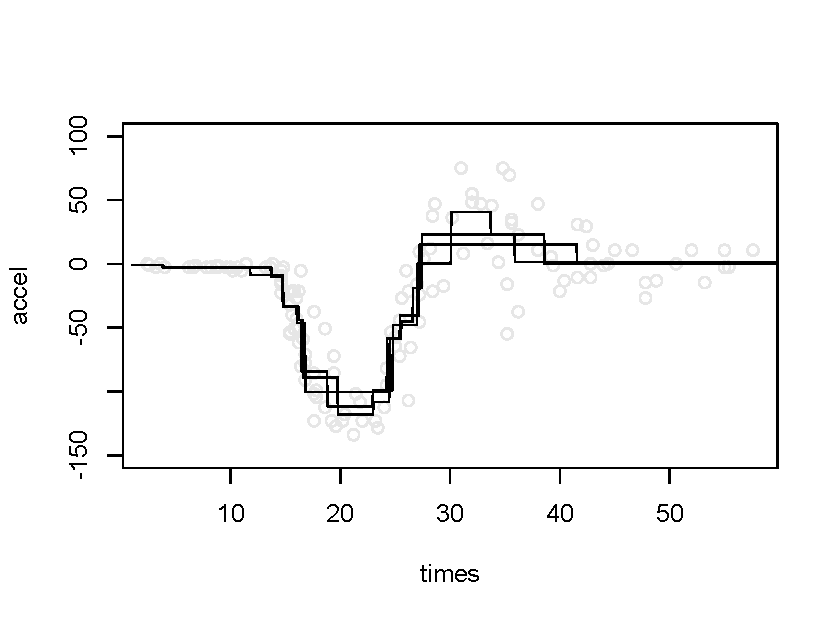
\includegraphics[width=4.25in]{../graphs/MCparticles}

\vskip -.25cm\sg
If you fit to random subsets of the data, \\\nv \hfill you get a slightly different
tree each time.
\vskip -.25cm
\end{frame}


\begin{frame}

{\bf  Model Averaging with \theme Random Forests}

\vskip .25cm
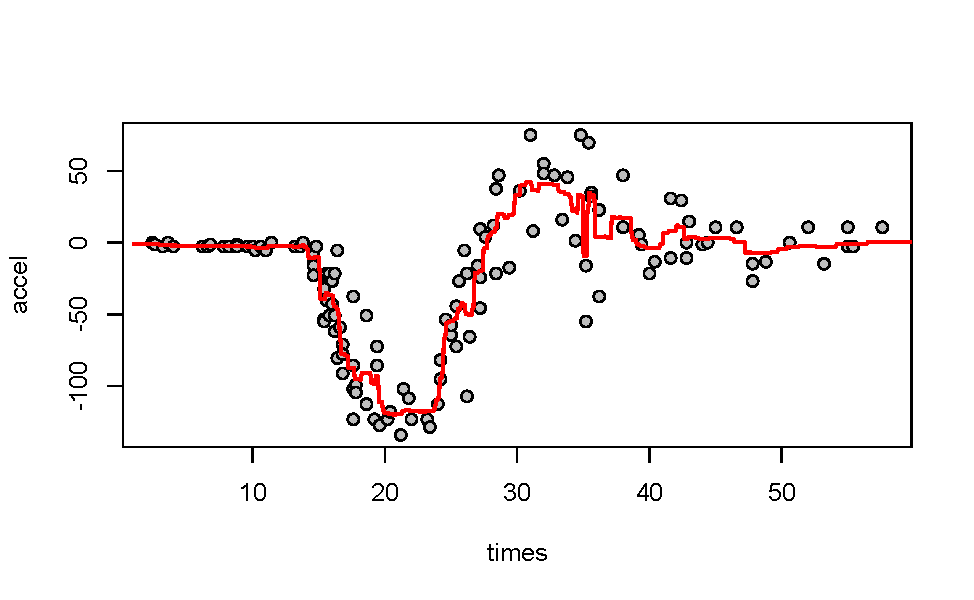
\includegraphics[width=4.35in]{../graphs/MCrf}

\vskip .2cm\sg
Averaging many trees yields a single
response surface. \\ \gr \it Still looks like a bit of overfit to me, which remains a
danger.

\vskip -.2cm

\end{frame}



\begin{frame}

{\bf A larger example: \theme California Housing Data}

\sk
Median home values in census tracts, along with
\begin{itemize}
\item Latitude and Longitude of tract centers.
\item Population totals and median income.
\item Average room/bedroom numbers, home age.
\end{itemize}
The goal is to predict {\nv log(MedVal)} for census tracts.


\sk
Difficult regression: \sg Covariate effects change with location.
\\\gr ~~~~~~~~~~~~~~~~~~~~~~~~~How they change is probably not linear.
\end{frame}


\begin{frame}

{\bf \theme CART Dendrogram for  CA housing}


\vspace{-1cm}
\begin{adjustwidth}{-.5in}{}
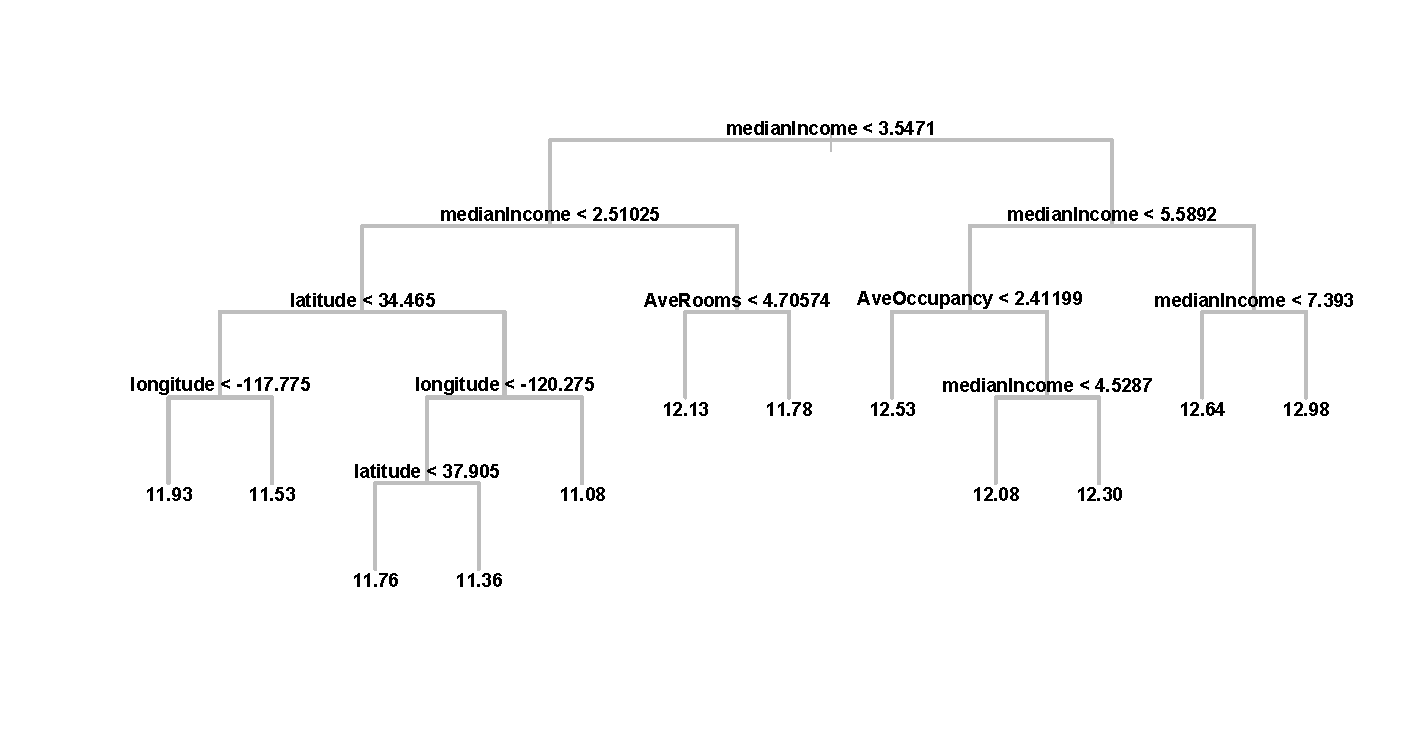
\includegraphics[width=5in]{../graphs/CAHtree}
\end{adjustwidth}

\vspace{-1cm}
\sg Income is dominant, with location important for low income.\\
\gr  Cross Validation favors the most complicated tree: 12 leaves.
\end{frame}


\begin{frame}

{\bf \theme LASSO \gr fit for CA housing data}

\vskip .2cm
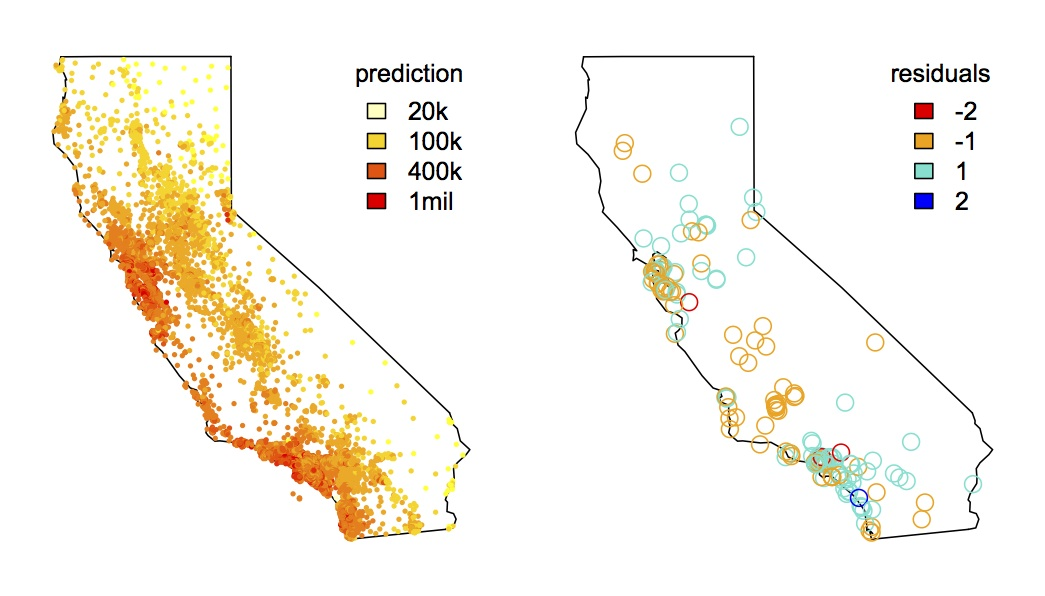
\includegraphics[width=4.25in]{../graphs/CAHlinpredSMALL}

\gr
Looks like over-estimates in the Bay, under-estimates in OC.
\end{frame}


\begin{frame}

{\bf \theme CART \gr fit for CA housing data}

\vskip .2cm
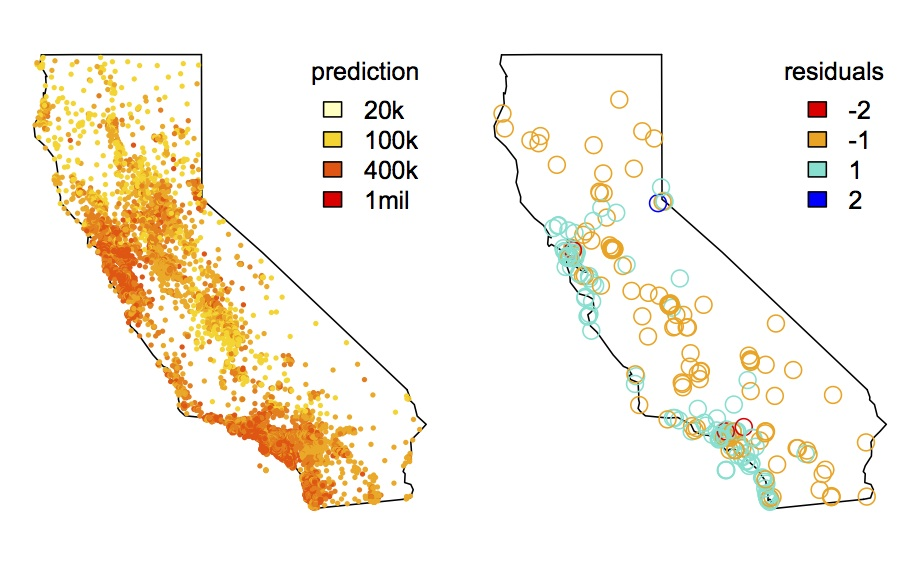
\includegraphics[width=4.25in]{../graphs/CAHtreepredSMALL}

\gr
Under-estimating the coast, over-estimating the central valley?
\end{frame}

\begin{frame}[fragile]

{\bf \theme randomForest \gr fit for CA housing data}

\vskip .2cm
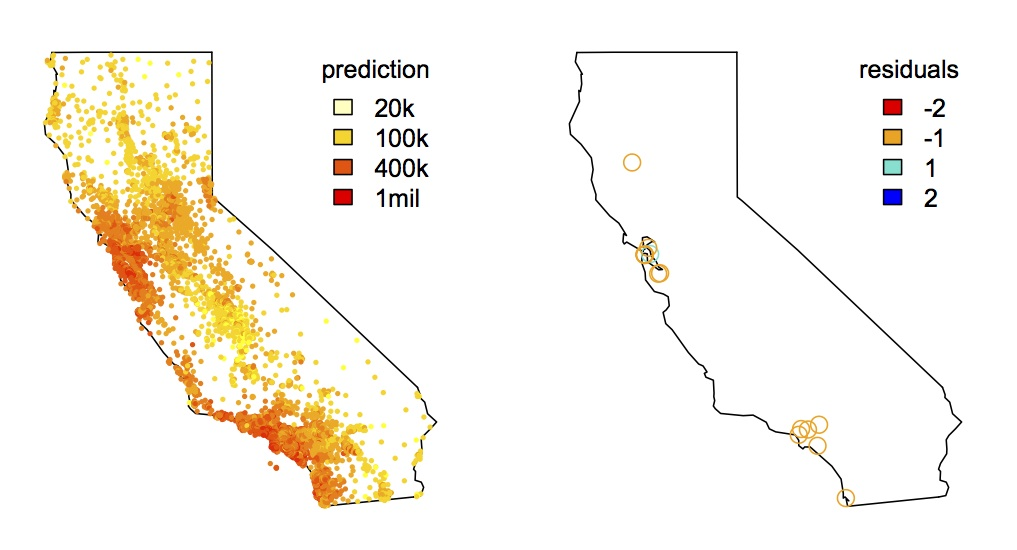
\includegraphics[width=4.25in]{../graphs/CAHrfpredSMALL}

No big residuals!  (although still missing the LA and SF effects)  \\\gr Overfit?  From out-of-sample prediction it
appears not.
\vskip -.15cm
\end{frame}

\begin{frame}

{\bf \theme CA housing: \bk out-of-sample prediction}

\vskip .5cm
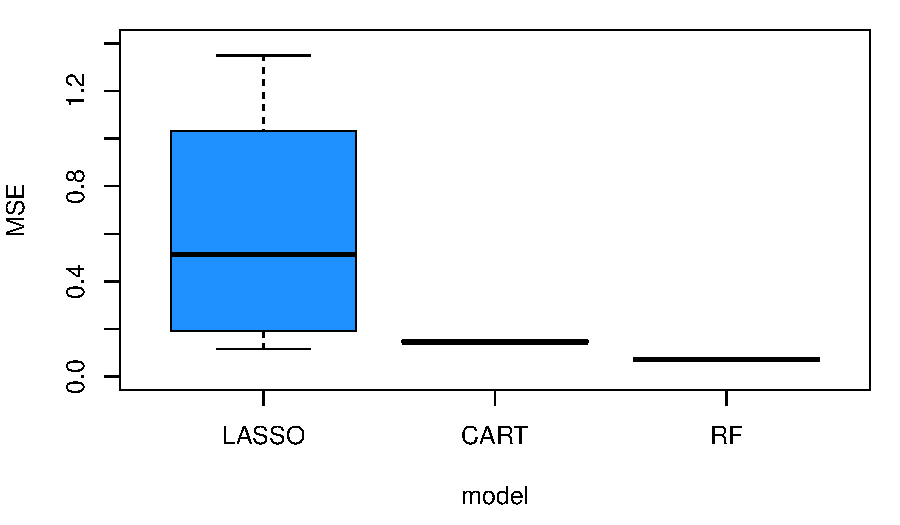
\includegraphics[width=4.25in]{../graphs/calhomesMSE}

Trees outperform LASSO:  ~gain from  nonlinear interaction.\\
RF is better still than CART: ~benefits of model averaging. 
\vskip -.25cm
\end{frame}


\begin{frame}




Although you don't have a nice single tree to interpret, {\tt
  randomForest} provides {\theme OOS} variable importance plots.

\vskip .2cm {\gr
You need to run randomForest with {\tt importance=TRUE}.  
Otherwise it doesn't store the necessary information.}


~~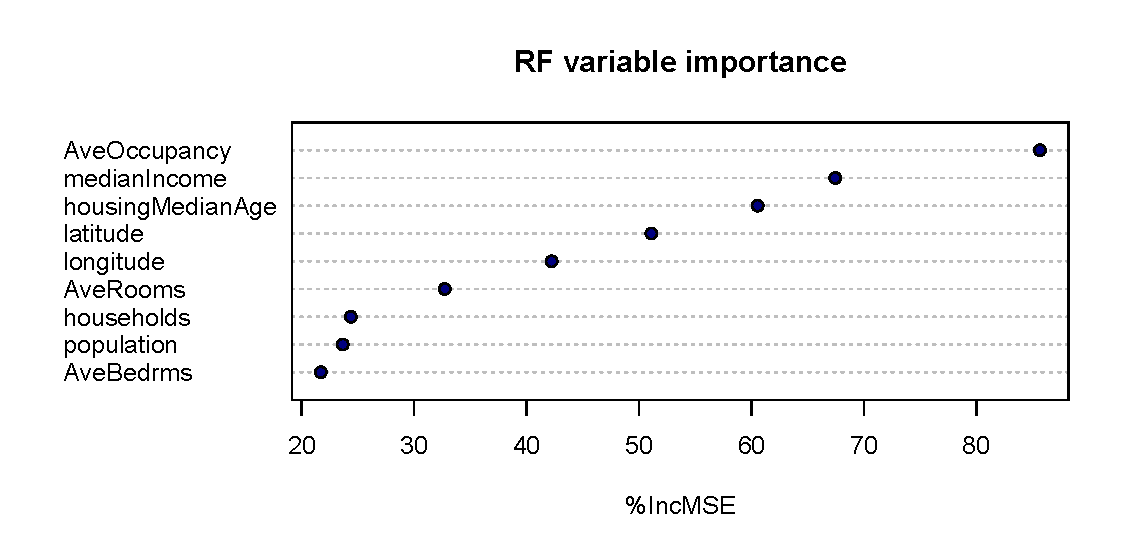
\includegraphics[width=3.85in]{../graphs/CAvarimp}

\vskip -.2cm
The $x$-axis here is the \% amount that
removing \\~~~splits on that variable would increase the MSE.\\
For classification it plots increase in \% misclassified.


\end{frame}

\begin{frame}

{\bf Roundup on  {\theme Tree-based learning}}

\vskip .25cm

We've seen two techniques for building tree models.
\begin{itemize}
\item {\nv CART:} recursive partitions, pruned back by CV.
\item {\nv randomForest:} average many simple CART trees.
\end{itemize}

\vskip .25cm
There are many other tree-based algorithms.
\begin{itemize}
\item {\nv Boosted Trees:} repeatedly fit simple trees to residuals.\\
{\gr Fast, but it is tough to avoid over-fit (requires full CV).}
\item {\nv Bayes Additive Regression Trees:} mix many simple trees.\\
{\gr Robust prediction, but suffers with non-constant variance.}
\item {\nv  Dynamic Trees:} grow  sequential `particle' trees\\
{\gr Good online, but fit depends on data ordering}
\end{itemize}

\vskip .25cm
{\bk Trees are poor in high dimension,  but fitting them to
low dimension factors (principle components) is a good option.}

\vskip -.2cm

\end{frame}

\begin{frame}

{\bf Roundup on  {\theme  Nonlinear Regression} and  {\theme  Classification}}


\vskip .25cm
Many other {\it nonparametric learning} algorithms
\begin{itemize}
\item Neural Networks (and deep learning):\\{\gr many recursive logistic
  regressions.}
\item Support Vector Machines: \\{\gr Project to HD, then
  classify.}
\item Gaussian Processes, splines, wavelets, etc: \\{\gr Use sums of curvy functions in regression.}
\end{itemize}

\vskip .25cm
Some of these are great, but all take a ton of tuning.

\vskip .25cm
{\theme Nothing's better out-of-the-box  in low dimension than trees.}
\nv
But: when the (simpler) linear model fits, it will do better. \\
\gr This is most often the case in very high dimension.
\end{frame}


\begin{frame}[fragile]
{Homework  due next week}

{Use your project data for this homework!  \\ {\gr If you don't have it yet, get it now.}}


\sk  {\it Build and interpret both a single tree and a random forest.}

\vskip .1cm
Compare the result to other techniques we've learned.

\vskip .1cm
~~~CART: fit, prune, {\tt +} plot.  Concentrate on interpretation.\\
~~~RF: plot variable importance and  predictive performance.\\

\sk {\gr [+]
{\it Use Random Forests in treatment effects estimation.}

\vskip .1cm
Look back to Lecture 4.  Replace lasso estimation for $\hat d(\bm{x})$ with a random forest.  Compare to the original two-lassos algorithm.}

\end{frame}

\end{document}
